%%=============================================================================
%% Inleiding
%%=============================================================================

\chapter{\IfLanguageName{dutch}{Inleiding}{Introduction}}%
\label{ch:inleiding}

De inleiding moet de lezer net genoeg informatie verschaffen om het onderwerp te begrijpen en in te zien waarom de onderzoeksvraag de moeite waard is om te onderzoeken. In de inleiding ga je literatuurverwijzingen beperken, zodat de tekst vlot leesbaar blijft. Je kan de inleiding verder onderverdelen in secties als dit de tekst verduidelijkt. Zaken die aan bod kunnen komen in de inleiding:

\begin{itemize}
  \item context, achtergrond
  \item afbakenen van het onderwerp
  \item verantwoording van het onderwerp, methodologie
  \item probleemstelling
  \item onderzoeksdoelstelling
  \item onderzoeksvraag
  \item \ldots
\end{itemize} 


\section{\IfLanguageName{dutch}{Probleemstelling}{Problem Statement}}%
\label{sec:probleemstelling}

\begin{figure}
  \centering
  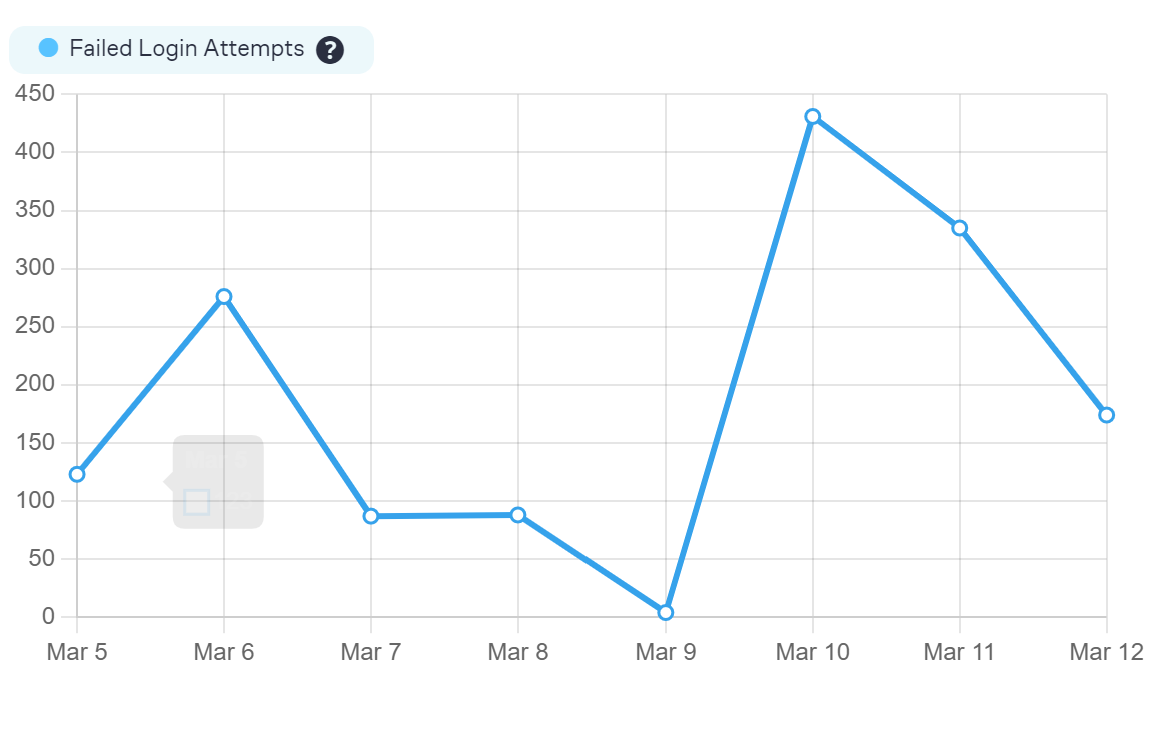
\includegraphics[height=0.3\textheight]{image.png}
  \caption[aantal aanvallen op de wordpress website van 24Flow per dag ]{aantal aanvallen op de wordpress website van 24Flow per dag }
\end{figure}
Kleine tot middelgrote IT-servicebedrijven, zoals Sinergio en 24Flow, worden dagelijks geconfronteerd met de uitdaging om hun 
webapplicaties effectief te beschermen tegen cyberaanvallen. Deze bedrijven maken vaak gebruik van populaire webontwikkelingsplatformen 
zoals WordPress en Laravel, die elk unieke beveiligingsrisico's en kwetsbaarheden kennen. De bescherming van deze platformen 
wordt vaak toevertrouwd aan de implementatie van beveiligingsplugins en -tools, waarvan de effectiviteit varieert.

Deze bachelorproef richt zich op het onderzoek naar de effectiviteit van verschillende penetratietesttools, zoals Burp Suite, Nmap en OWASP ZAP, 
in het identificeren van kwetsbaarheden binnen drie specifieke webomgevingen: een WordPress applicatie zonder beveiligingsplugins,
een WordPress applicatie met beveiligingsplugins en een afgewerkte Laravel applicatie. Het doel van dit onderzoek is tweeledig: 
ten eerste het vaststellen van de meest effectieve penetratietesttool(s) voor deze specifieke webomgevingen. Ten tweede het 
analyseren van de beveiligingsrisico's geassocieerd met elk van deze omgevingen om de vraag te beantwoorden hoe onveilig een 
WordPress applicatie zonder beveiligingsplugins werkelijk is. Dit wordt vergeleken met een WordPress applicatie met 
beveiligingsplugins en een Laravel applicatie.

De directe doelgroep voor deze bachelorproef is het bedrijf Sinergio, een kleine IT-serviceprovider die regelmatig 
werkt met WordPress en Laravel voor het ontwikkelen van webapplicaties voor hun klanten. De resultaten van dit 
onderzoek bieden Sinergio waardevolle inzichten in de meest effectieve manieren om hun webontwikkelingsprojecten 
te beveiligen. Dit stelt hen in staat om geïnformeerde beslissingen te nemen over de implementatie van 
beveiligingsstrategieën en -tools. Bovendien draagt dit onderzoek bij aan een bredere kennisbasis over webapplicatiebeveiliging, 
wat van belang kan zijn voor andere kleine tot middelgrote IT-bedrijven die vergelijkbare technologieën gebruiken.

\section{\IfLanguageName{dutch}{Onderzoeksvraag}{Research question}}%
\label{sec:onderzoeksvraag}
Hoe variëren de prestaties van verschillende penetratietesttools bij het identificeren van kwetsbaarheden binnen drie 
specifieke webomgevingen: een WordPress-website zonder beveiligingsplugins, een WordPress-website met beveiligingsplugins 
en een volledig ontwikkelde Laravel-applicatie? Welke specifieke kwetsbaarheden detecteren de penetratietesttools in een WordPress-omgeving zonder 
beveiligingsplugins en hoe verschilt dit van de omgevingen met beveiligingsplugins en de Laravel-applicatie? 
In hoeverre verbeteren beveiligingsplugins de detectiecapaciteiten van deze tools op een WordPress-site? 
Tot slot zal je onderzoek de beveiligingsniveaus van een onbeveiligde WordPress-website vergelijken met die 
van een beveiligde site en een Laravel-applicatie, om zo te bepalen hoe de aanwezigheid van beveiligingsplugins de 
veiligheid beïnvloedt.

\section{\IfLanguageName{dutch}{Onderzoeksdoelstelling}{Research objective}}%
\label{sec:onderzoeksdoelstelling}
De doelstelling is het uitvoeren van een vergelijkende studie. Deze studie evalueert de effectiviteit van 
verschillende penetratietesttools bij het identificeren van kwetsbaarheden in drie specifieke webomgevingen: een WordPress-website 
zonder beveiligingsplugins, een WordPress-website met beveiligingsplugins en een volledig ontwikkelde Laravel-applicatie.
Het beoogde resultaat is een verslag met gedetailleerde aanbevelingen over de meest effectieve tools voor elke geteste 
omgeving. Het succes wordt gemeten aan de hand van de volledigheid van de verzamelde data, de analytische diepgang van de bevindingen, 
en de duidelijkheid van de vergelijkende analyse tussen de tools en omgevingen. Dit verslag zal essentiële inzichten bieden die 
bijdragen aan betere beveiligingsstrategieën en -implementaties in webontwikkelingsprojecten.
\section{\IfLanguageName{dutch}{Opzet van deze bachelorproef}{Structure of this bachelor thesis}}%
\label{sec:opzet-bachelorproef}

% Het is gebruikelijk aan het einde van de inleiding een overzicht te
% geven van de opbouw van de rest van de tekst. Deze sectie bevat al een aanzet
% die je kan aanvullen/aanpassen in functie van je eigen tekst.

De rest van deze bachelorproef is als volgt opgebouwd:

In Hoofdstuk~\ref{ch:stand-van-zaken} wordt een overzicht gegeven van de stand van zaken binnen het onderzoeksdomein, op basis van een literatuurstudie.

In Hoofdstuk~\ref{ch:methodologie} wordt de methodologie toegelicht en worden de gebruikte onderzoekstechnieken besproken om een antwoord te kunnen formuleren op de onderzoeksvragen.

% TODO: Vul hier aan voor je eigen hoofstukken, één of twee zinnen per hoofdstuk
In Hoofdstuk~\ref{ch:resultaten}, bevat de resultaten van het onderzoek.

In Hoofdstuk~\ref{ch:conclusie}, tenslotte, wordt de conclusie gegeven en een antwoord geformuleerd op de onderzoeksvragen. Daarbij wordt ook een aanzet gegeven voor toekomstig onderzoek binnen dit domein.